\subsection{Tipo de entidad Calificación Convocatoria}

   \begin{description}

   \item[Definición] Se refiere al objeto del mundo real: \emph{``Calificacón
   obtenida por un alumno en una determinada convocatoria de una asignatura''}.

   \item[Características] La entidad presenta las siguientes características:
      \begin{itemize}
         \item \textbf{Nombre:} Calificación Convocatoria.
         \item \textbf{Tipo:} Débil por identificación con respecto a las
         entidades Alumno Curso Académico y Asignatura Curso Académico.
         \item \textbf{Número de atributos:} 3 propios y 5 heredados.
         \item \textbf{Atributo/s identificador/es principal/es:} id\_centro
         junto con \newline id\_titulación, id\_asignatura, curso\_académico,
         dni\_pasaporte y convocatoria.
         \item \textbf{Atributo/s identificador/es alternativo/s:} -
         \item \textbf{Atributo/s heredado/s:} id\_centro, id\_titulación,
         id\_asignatura, \newline curso\_académico y dni\_pasaporte del tipo de
         entidad Matrícula.
         \item \textbf{Información adicional:} -
      \end{itemize}

   \item[Diagrama] La figura \ref{diagramaCalConv} muestra el diagrama de la
   entidad.
   \item \begin{figure}[!ht]
            \begin{center}
            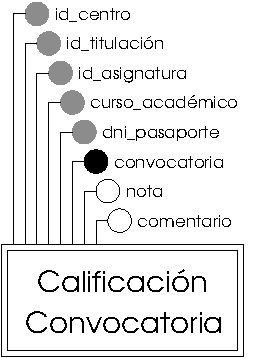
\includegraphics[]{07.Modelo_Entidad-Interrelacion/7.2.Analisis_Entidades/diagramas/cal_conv.pdf}
            \caption{Diagrama de la entidad Calificación Convocatoria.}
            \label{diagramaCalConv}
            \end{center}
         \end{figure}

   \item[Descripción de los atributos propios] La entidad presenta los
   siguientes atributos propios:

   \begin{itemize}
    \item \textbf{convocatoria}
     \begin{itemize}
       \item \textbf{Definición:} Establece la convocatoria en la que el
       alumno se presenta a la asignatura.
       \item \textbf{Dominio:} Conjunto de caracteres alfanuméricos.
       \item \textbf{Carácter:} Obligatorio.
       \item \textbf{Ejemplo práctico:} febrero.
       \item \textbf{Información adicional:} Forma parte de la clave primaria de
       la entidad. El dato lo introduce el usuario alumno al actualizar
       su información personal, o bien el usuario asesor si
       comprueba que la información no es correcta.
     \end{itemize}
     \item \textbf{nota}
     \begin{itemize}
       \item \textbf{Definición:} Establece la calificación obtenida por un
       alumno en una convocatoria de una asignatura.
       \item \textbf{Dominio:} Conjunto de reales positivos.
       \item \textbf{Carácter:} Opcional.
       \item \textbf{Ejemplo práctico:} 8,4.
       \item \textbf{Información adicional:} El dato lo introduce el
       usuario alumno al actualizar su información personal , o
       bien el usuario asesor si comprueba que la información no es
       correcta.
     \end{itemize}
    \item \textbf{comentario}
    \begin{itemize}
      \item \textbf{Definición:} Información extra que pueda ser
      interesante conocer.
      \item \textbf{Dominio:} Conjunto de caracteres alfanuméricos.
      \item \textbf{Carácter:} Opcional.
      \item \textbf{Ejemplo práctico:} Prácticas superadas.
      \item \textbf{Información adicional:} El dato lo introduce el
      usuario alumno al actualizar su información personal , o
      bien el usuario asesor si comprueba que la información no es
      correcta.
    \end{itemize}
   \end{itemize}

   \item[Ejemplo práctico]

   \item \begin{center}
            \begin{tabular}{ | l | l | }
            \hline
            \multicolumn{2}{ | c | }{\textbf{Tipo de entidad Calificación
            Convocatoria}} \\
            \hline
            id\_centro & 15 \\
            \hline
            id\_titulación & 3\\
            \hline
            id\_asignatura & 17\\
            \hline
            curso\_académico & 2008 \\
            \hline
            dni\_pasaporte & 01234567A \\
            \hline
            convocatoria & febrero \\
            \hline
            nota & 8,4 \\
            \hline
            comentario & Prácticas superadas \\
            \hline
            \end{tabular}
         \end{center}
   \end{description}
